
\section{A/D převodníky}
Analogově-digitální převodník je elektronická součástka určená k převodu analogového (spojitého) signálu na signál digitální (diskrétní). Důvodem převodu je umožnit zpracování analogového signálu na číslicových počítačích.

\subsection{Analogový a digitální signál}

\paragraph{Analogový signál}
Analogový signál je dán spojitou funkcí času. Má teoreticky nekonečné množství hodnot. S opakovanou rekonstrukcí ztrácí na kvalitě.

\paragraph{Diskrétní signál}
Diskrétní signál je dán funkcí definovanou pouze v diskrétních (nespojitých) časových intervalech. To znamená že jeho okamžitá hodnota se nemění spojitě s časem. Pokud se hodnota signálu mění pouze v izolovaných okamžicích, mluvíme o vzorkovaném signálu. Pokud signál může nabývat v libovolném okamžiku pouze jednu z konečného počtu hodnot, mluvíme o signálu kvantovaném. V praxi se obě metody kombinují, a výsledný signál se nazýva digitální.

\paragraph{Vzorkovaný signál}
Vzorkovaný signál je signál, který není spojitý v čase. Je tvořen posloupností vzorků, které obecně mohou nabývat libovolnou hodnotu. Tento signál vzniká vzorkováním analogového signálu, přičemž počet vzorků za sekundu udává vzorkovací kmitočet. 
\begin{figure}[htbp]
\centering
\includesvg[scale=0.5]{sections/5_ad_prevodiky/images/Sampled.signal.svg}
\end{figure}
\paragraph{Kvantovaný signál}
Kvantovaný (kvantizovaný) signál je signál, jehož hodnota nemá spojitý průběh, ale mění se skokem, přičemž nabývá pouze omezeného počtu úrovní. Ke změně hodnoty signálu může obecně dojít v libovolném čase. Tento signál vzniká obvykle kvantováním analogového signálu.  Příliš malý počet kvantizačních úrovní se projeví jako tak zvaný kvantizační šum, který je dán rozdílem kvantovaného signálu a původního signálu.
\begin{figure}[htbp]
\centering
\includesvg[scale=0.5]{sections/5_ad_prevodiky/images/Quantized.signal.svg}
\end{figure}
\paragraph{Digitální signál}
Digitální signál (též číslicový signál) je signál, který je vzorkovaný a následně kvantovaný. Je tvořen posloupností vzorků, které mohou nabývat pouze omezeného počtu hodnot, takže jej lze reprezentovat posloupností celých čísel. Při převodu analogového signálu na digitální vždy dochází ke ztrátě informace (jak při vzorkování tak při kvantování). Zvyšováním vzorkovacího kmitočtu a počtu úrovní kvantizace se však lze k původnímu signálu přiblížit s libovolně malou odchylkou.
\begin{figure}[htbp]
\centering
\includesvg[scale=0.5]{sections/5_ad_prevodiky/images/Digital.signal.svg}
\end{figure}
\paragraph{Rozdíl mezi digitálním a diskrétním signálem} 
Diskrétní signál je širší pojem, který zahrnuje všechny signály vzorkované v diskrétních časových okamžicích. Digitální signál je speciální typ diskrétního signálu, kde jsou hodnoty kvantizovány na určité množství úrovní, obvykle reprezentovaných binárními čísly.

\subsection{Převod A/D signálu}

\subsubsection{Vzorkování}
Úsek spojitého signálu se sice dá donekonečna zvětšovat a pozorovat tak jeho nekonečně malé detaily, ale protože počítače mají pouze konečnou kapacitu paměti a ani nejsou nekonečně rychlé, musíme se u reálného vzorkování při A/D převodu omezit na nezbytně nutné množství vzorků, které budeme dále zpracovávat.
Vzorkování se provede tím způsobem, že rozdělíme vodorovnou osu signálu (čas) na rovnoměrné úseky a z každého úseku odebereme jeden vzorek. Je přitom zřejmé, že tak z původního signálu ztratíme mnoho detailů, protože namísto spojité čáry, kterou lze donekonečna zvětšovat, dostáváme pouze množinu diskrétních bodů s intervalem odpovídajícím použité vzorkovací frekvenci.

\paragraph{Shonnon-Nyquistův-Kotělnikovův teorém}
Podle Shannon-Nyquistova teorému musí být vzorkovací kmitočet nejméně dvakrát větší než je nejvyšší přenášený kmitočet.

\paragraph{Aliasing}
Aliasing je jev, který vzniká při vzorkování signálu pod Nyquistovou frekvencí.

\subsubsection{Kvantování}
Vzhledem k tomu, že počítače a další zařízení dále zpracovávající digitální signál umí vyjádřit čísla pouze s omezenou přesností, je třeba navzorkované hodnoty upravit i na svislé ose. Protože se hodnota vzorku dá vyjádřit pouze po určitých kvantech, nazýváme tuto fázi A/D převodu kvantování. Veličina na svislé ose může nabývat pouze určitých hodnot. Aby bylo možné určit, které hodnoty má po kvantování nabývat určitý vzorek, je třeba rozdělit prostor kolem jednotlivých hodnot na toleranční pásy. Kterémukoli vzorku, který padne do daného tolerančního pásu, je při kvantování přiřazena daná hodnota. Kvantované hodnoty se ve většině případů liší od skutečných navzorkovaných hodnot. Velikost kvantizační chyby je vzdálenost mezi kvantovanými a původními navzorkovanými body. Velikost této chyby se pohybuje v intervalu +1/2 až -1/2 kvantizační úrovně. 

\paragraph{Kvantizační šum}
Při vynešení velikosti chyb od jednotlivých vzorků do grafu se získá náhodný signál, kterému se říká kvantizační šum. Velikost šumu je zvykem vyjadřovat jako poměrné číslo v decibelech, a sice jako poměr užitečného signálu k šumu
\subsection{Druhy převodníků}

\subsubsection{Paralelní}
Paralelní A/D převodník je nejrychlejším typem A/D převodníku, protože převod probíhá v jednom časovém okamžiku. Kvantování vstupního signálu se vyjadřuje v komparátorech, které porovnávají vstupní napětí s odstupňovaným referenčním napětím (vytváří se v odporové síti). Převodník s rozlišitelností n bitů obsahuje $2^n-1$ komparátorů. Vzorkování vstupního signálu se uskutečňuje zápisem stavu výstupů komparátorů do klopných obvodů (příchodem hodinového impulsu). Dekodér je kombinační obvod, který převádí informaci o výstupech komparátorů na určitý kód.
\begin{figure}[htbp]
\centering
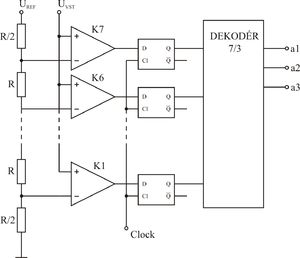
\includegraphics[scale=3]{sections/5_ad_prevodiky/images/300px-Komparacni_AD_prevodnik.png}
\end{figure}
\subsubsection{Přírůstkový}
Na začátku cyklu se spuštěním signálu start vynuluje čítač. Na vstupu je připojeno napětí, na výstupu komparátoru je log1 a do čítače začnou přes hradlo AND procházet impulsy z generátoru, obsah čítače se s krokem LSB zvyšuje; z výstupu čítače jde také signál do zpětnovazební větve, ve které je zapojen číslicově-analogový převodník. Napětí na výstupu D/A převodníku se postupně zvyšuje. Dosáhne-li toto napětí hodnoty vstupního napětí, překlopí se komparátor do stavu L, tím se uzavře hradlo, přeruší se impuls v generátoru, čítání se zastaví a do paměti se zapíše platné výstupní slovo. Další čítací impuls se provede signálem start.
\begin{figure}[htbp]
\centering
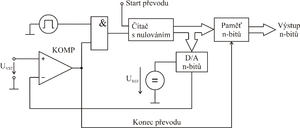
\includegraphics[scale=3]{sections/5_ad_prevodiky/images/300px-Kompenzacni_citaci_AD.png}
\end{figure}
\subsubsection{S vratným čítačem}
Má stejný princip jako čítací, pouze je použit obousměrný čítač, který může čítat vpřed i vzad. Napěťový komparátor řídí směr čítání, takže číslicový výstup sleduje změny vstupního napětí. Patří mezi často používané převodníky. U čítacího a sledovacího převodníku se v každém taktu generátoru hodinových impulsů mění slova vždy o hodnotu LSB.

\subsubsection{S postupnou aproximací}
Při použití postupné aproximace se zkusmo nastaví jednotlivé váhové bity. Začíná se bitem MSB a končí bitem LSB. Na začátku cyklu převodu se nastaví hodnota převodu výstupu aproximačního registru na 10000000, čemuž odpovídá výstup zpětnovazebního D/A převodníku UREF/2. Toto napětí se porovnává v komparátoru s vstupním napětím. Je-li UVST větší než UREF/2, ponechá se MSB nastaven na 1, v opačném případě se vrátí na 0. V druhém kroku se zkusmo nastaví na 1 další váhový bit. Na výstupu tedy bude 11000000 nebo 01000000, podle výsledku předchozího kroku. Opět se porovná zpětnovazební a vstupní napětí a aktuální bit se nastaví na 1 nebo se vrátí na 0, takto se postupuje až k LSB. V tomto převodníku je doba převodu nižší než v čítacím převodníku a je nezávislá na vstupním napětí. Změna vstupního napětí během převodu způsobí chybu, a proto na rozdíl od čítacího převodníku musí být vstup opatřen vzorkovacím obvodem. Převodníky se vyrábějí 8bitové a 16bitové.
\begin{figure}[htbp]
\centering
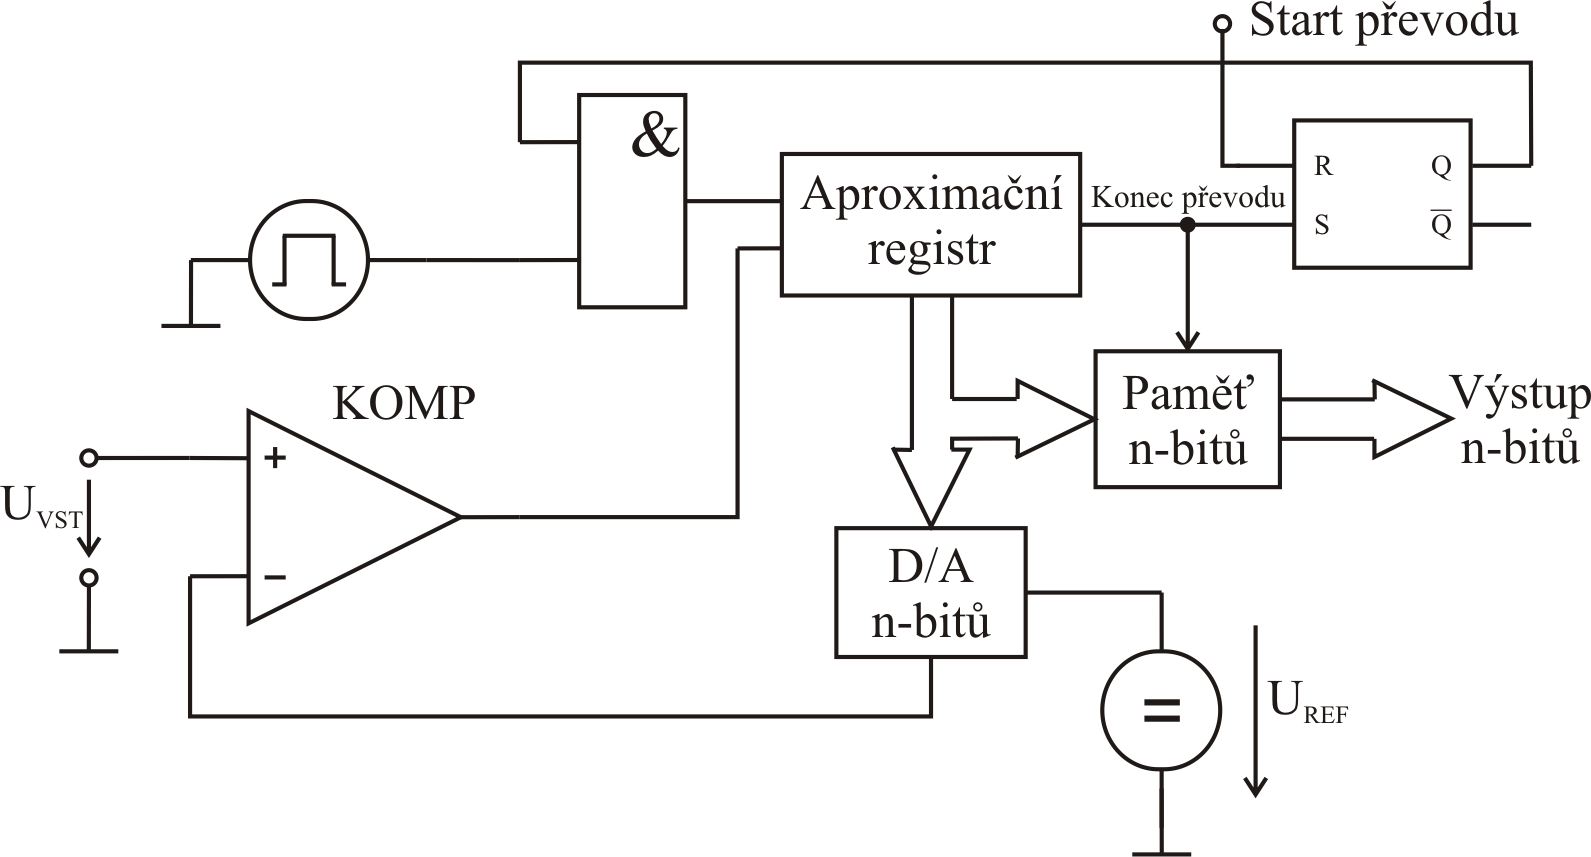
\includegraphics[scale=0.5]{sections/5_ad_prevodiky/images/Kompenzacni_sledovaci_AD.png}
\end{figure}
\subsubsection{S dvojitou integrací}
Tento typ převodníku se často používá v multimetrech. Vlastní převod probíhá ve dvou taktech. Na začátku měřicího cyklu je integrační kondenzátor vybitý a čítač vynulovaný. V prvním taktu je na vstup integrátoru přivedeno vstupní napětí a čítač čítá impulsy krystalového generátoru. Absolutní hodnota napětí na integrátoru se zvyšuje se strmostí danou velikostí vstupního napětí. Tento děj probíhá tak dlouho, dokud nedojde k zaplnění čítače (přetečení). V okamžiku přetečení čítače (všechny výstupy jsou ve stavu L) je zahájen druhý takt, přepne se přepínač a na vstup integrátoru se připojí referenční napětí opačné polarity, než je vstupní napětí. Absolutní hodnota výstupního napětí integrátoru se zmenšuje. Jakmile dosáhne nulové hodnoty, překlopí komparátor a tím se ukončí převod. Výhodou převodníku s dvojitou integrací je, že je eliminován vliv časové nestability RC prvků integrátoru a kmitočtu oscilátoru. Důležitá je přesnost a stabilita referenčního napětí.
\begin{figure}[htbp]
\centering
\includegraphics[scale=0.5]{sections/5_ad_prevodiky/images/AD_s_dvoutaktní_integraci.png}
\end{figure}
\subsubsection{Sigma-delta}
Umožňují dosáhnout velmi vysoké linearity převodu při vysokém rozlišení, až 24 bitů. Rychlost převodu je však nižší. Lze digitalizovat v pásmu do desítek kHz – nízkofrekvenční pásmo. Převodník se skládá ze sigma-delta modulátoru a číslicového filtru. Základními obvody modulátoru jsou dolní propust (integrátor), napěťový komparátor a klopný obvod typu D, překlápěný hodinovým signálem s frekvencí f0. Dále je zde zpětnovazební větev s jednobitovým D/A převodníkem, což je vlastně přepínač dvouhodnotového signálu UREF. Tento signál se odečítá od vstupního napětí v rozdílovém zesilovači. U převodníku vzniká kvantizační šum, který je rovnoměrně rozložen v pásmu spektra frekvencí od 0 do f0/2, jestliže u číslicového filtru vzorkujeme frekvencí f0/K, kde K se nazývá koeficient nevzorkování (bývá 10–104), sníží se efektivní výkon kvantizačního šumu a dojde ke zvýšení efektivního počtu převodníku. Sigma-delta převodníky se hodí k měření stejnosměrných nebo pomalu se měnících napětí.
\begin{figure}[htbp]
\centering
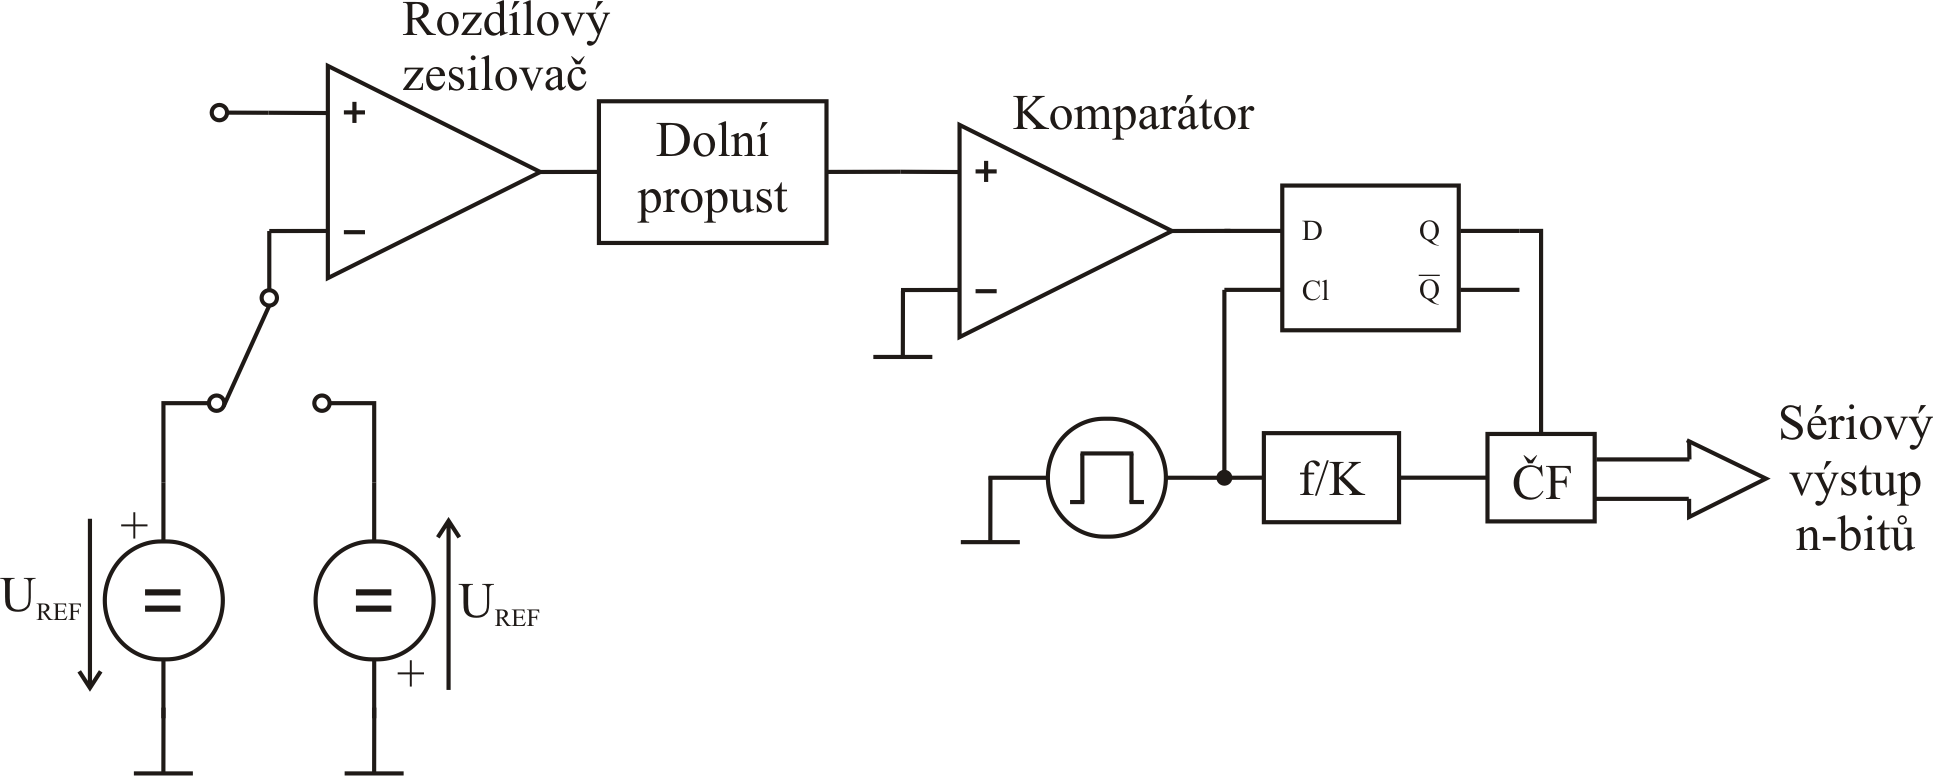
\includegraphics[scale=0.5]{sections/5_ad_prevodiky/images/Sigma-delta_prevodnik.png}
\end{figure}
